\documentclass[twoside]{book}

% Packages required by doxygen
\usepackage{fixltx2e}
\usepackage{calc}
\usepackage{doxygen}
\usepackage[export]{adjustbox} % also loads graphicx
\usepackage{graphicx}
\usepackage[utf8]{inputenc}
\usepackage{makeidx}
\usepackage{multicol}
\usepackage{multirow}
\PassOptionsToPackage{warn}{textcomp}
\usepackage{textcomp}
\usepackage[nointegrals]{wasysym}
\usepackage[table]{xcolor}

% Font selection
\usepackage[T1]{fontenc}
\usepackage[scaled=.90]{helvet}
\usepackage{courier}
\usepackage{amssymb}
\usepackage{sectsty}
\renewcommand{\familydefault}{\sfdefault}
\allsectionsfont{%
  \fontseries{bc}\selectfont%
  \color{darkgray}%
}
\renewcommand{\DoxyLabelFont}{%
  \fontseries{bc}\selectfont%
  \color{darkgray}%
}
\newcommand{\+}{\discretionary{\mbox{\scriptsize$\hookleftarrow$}}{}{}}

% Page & text layout
\usepackage{geometry}
\geometry{%
  a4paper,%
  top=2.5cm,%
  bottom=2.5cm,%
  left=2.5cm,%
  right=2.5cm%
}
\tolerance=750
\hfuzz=15pt
\hbadness=750
\setlength{\emergencystretch}{15pt}
\setlength{\parindent}{0cm}
\setlength{\parskip}{3ex plus 2ex minus 2ex}
\makeatletter
\renewcommand{\paragraph}{%
  \@startsection{paragraph}{4}{0ex}{-1.0ex}{1.0ex}{%
    \normalfont\normalsize\bfseries\SS@parafont%
  }%
}
\renewcommand{\subparagraph}{%
  \@startsection{subparagraph}{5}{0ex}{-1.0ex}{1.0ex}{%
    \normalfont\normalsize\bfseries\SS@subparafont%
  }%
}
\makeatother

% Headers & footers
\usepackage{fancyhdr}
\pagestyle{fancyplain}
\fancyhead[LE]{\fancyplain{}{\bfseries\thepage}}
\fancyhead[CE]{\fancyplain{}{}}
\fancyhead[RE]{\fancyplain{}{\bfseries\leftmark}}
\fancyhead[LO]{\fancyplain{}{\bfseries\rightmark}}
\fancyhead[CO]{\fancyplain{}{}}
\fancyhead[RO]{\fancyplain{}{\bfseries\thepage}}
\fancyfoot[LE]{\fancyplain{}{}}
\fancyfoot[CE]{\fancyplain{}{}}
\fancyfoot[RE]{\fancyplain{}{\bfseries\scriptsize Generated by Doxygen }}
\fancyfoot[LO]{\fancyplain{}{\bfseries\scriptsize Generated by Doxygen }}
\fancyfoot[CO]{\fancyplain{}{}}
\fancyfoot[RO]{\fancyplain{}{}}
\renewcommand{\footrulewidth}{0.4pt}
\renewcommand{\chaptermark}[1]{%
  \markboth{#1}{}%
}
\renewcommand{\sectionmark}[1]{%
  \markright{\thesection\ #1}%
}

% Indices & bibliography
\usepackage{natbib}
\usepackage[titles]{tocloft}
\setcounter{tocdepth}{3}
\setcounter{secnumdepth}{5}
\makeindex

% Hyperlinks (required, but should be loaded last)
\usepackage{ifpdf}
\ifpdf
  \usepackage[pdftex,pagebackref=true]{hyperref}
\else
  \usepackage[ps2pdf,pagebackref=true]{hyperref}
\fi
\hypersetup{%
  colorlinks=true,%
  linkcolor=blue,%
  citecolor=blue,%
  unicode%
}

% Custom commands
\newcommand{\clearemptydoublepage}{%
  \newpage{\pagestyle{empty}\cleardoublepage}%
}

\usepackage{caption}
\captionsetup{labelsep=space,justification=centering,font={bf},singlelinecheck=off,skip=4pt,position=top}

%===== C O N T E N T S =====

\begin{document}

% Titlepage & ToC
\hypersetup{pageanchor=false,
             bookmarksnumbered=true,
             pdfencoding=unicode
            }
\pagenumbering{roman}
\begin{titlepage}
\vspace*{7cm}
\begin{center}%
{\Large Voting System }\\
\vspace*{1cm}
{\large Generated by Doxygen 1.8.11}\\
\end{center}
\end{titlepage}
\clearemptydoublepage
\tableofcontents
\clearemptydoublepage
\pagenumbering{arabic}
\hypersetup{pageanchor=true}

%--- Begin generated contents ---
\chapter{Team 13 Index Page}
\label{index}\hypertarget{index}{}\hypertarget{index_intro_sec}{}\section{Introduction}\label{index_intro_sec}
VS is a voting system designed to implement both plurality voting as well as single transferable voting (\mbox{\hyperlink{class_s_t_v}{S\+TV}}) methods. \mbox{\hyperlink{class_election}{Election}} holders are able to select the parameters of the election (ie. number of candidates, number of available seats, and number of ballots cast) as well as the desired voting method. The system will then assign winners to the available seats. 
\chapter{Hierarchical Index}
\section{Class Hierarchy}
This inheritance list is sorted roughly, but not completely, alphabetically\+:\begin{DoxyCompactList}
\item \contentsline{section}{Ballot}{\pageref{class_ballot}}{}
\item \contentsline{section}{Ballot\+List}{\pageref{class_ballot_list}}{}
\item \contentsline{section}{Candidate}{\pageref{class_candidate}}{}
\item \contentsline{section}{Candidate\+List}{\pageref{class_candidate_list}}{}
\item \contentsline{section}{Election}{\pageref{class_election}}{}
\begin{DoxyCompactList}
\item \contentsline{section}{Plurality}{\pageref{class_plurality}}{}
\item \contentsline{section}{S\+TV}{\pageref{class_s_t_v}}{}
\end{DoxyCompactList}
\item \contentsline{section}{main}{\pageref{classmain}}{}
\end{DoxyCompactList}

\chapter{Class Index}
\section{Class List}
Here are the classes, structs, unions and interfaces with brief descriptions\+:\begin{DoxyCompactList}
\item\contentsline{section}{\mbox{\hyperlink{class_ballot}{Ballot}} \\*An object containing the voting ballots }{\pageref{class_ballot}}{}
\item\contentsline{section}{\mbox{\hyperlink{class_ballot_list}{Ballot\+List}} \\*An object containing a list of Ballots }{\pageref{class_ballot_list}}{}
\item\contentsline{section}{\mbox{\hyperlink{class_candidate}{Candidate}} \\*An object representing a \mbox{\hyperlink{class_candidate}{Candidate}} }{\pageref{class_candidate}}{}
\item\contentsline{section}{\mbox{\hyperlink{class_candidate_list}{Candidate\+List}} \\*An object containing a list of candidates }{\pageref{class_candidate_list}}{}
\item\contentsline{section}{\mbox{\hyperlink{class_election}{Election}} \\*An object that receives information about the number of seats, candidates, and ballots. Likewise, the class will store objects of \mbox{\hyperlink{class_candidate_list}{Candidate\+List}} and \mbox{\hyperlink{class_ballot_list}{Ballot\+List}} }{\pageref{class_election}}{}
\item\contentsline{section}{\mbox{\hyperlink{classmain}{main}} \\*Main driver of the Voting System }{\pageref{classmain}}{}
\item\contentsline{section}{\mbox{\hyperlink{class_plurality}{Plurality}} \\*Inherits from the \mbox{\hyperlink{class_election}{Election}} class. The class implements the \mbox{\hyperlink{class_plurality}{Plurality}} algorithm to identify the winning candidates }{\pageref{class_plurality}}{}
\item\contentsline{section}{\mbox{\hyperlink{class_s_t_v}{S\+TV}} \\*Inherits from the \mbox{\hyperlink{class_election}{Election}} class. The class implements the \mbox{\hyperlink{class_s_t_v}{S\+TV}} algorithm to identify the winning candidates }{\pageref{class_s_t_v}}{}
\end{DoxyCompactList}

\chapter{Class Documentation}
\hypertarget{class_ballot}{}\section{Ballot Class Reference}
\label{class_ballot}\index{Ballot@{Ballot}}


An object containing the voting ballots.  




{\ttfamily \#include $<$Ballot.\+h$>$}

\subsection*{Public Member Functions}
\begin{DoxyCompactItemize}
\item 
\hyperlink{class_ballot_af9078126260b3f58ea91f6b82797396b}{Ballot} ()
\item 
\hyperlink{class_ballot_afdbfa652a622a1d5aad8ec911a29a91f}{Ballot} (int num, std\+::vector$<$ int $>$ vote)
\begin{DoxyCompactList}\small\item\em Creates a ballot that contains the ballot number and the voters corresponding votes. \end{DoxyCompactList}\item 
int \hyperlink{class_ballot_ae68cc4486852163b21b85d0b96916a5e}{get\+\_\+ballot\+\_\+no} ()\hypertarget{class_ballot_ae68cc4486852163b21b85d0b96916a5e}{}\label{class_ballot_ae68cc4486852163b21b85d0b96916a5e}

\begin{DoxyCompactList}\small\item\em Gets the ballot number from the class. \end{DoxyCompactList}\item 
int {\bfseries get\+\_\+current} ()\hypertarget{class_ballot_a0a0775b462086988e8fc43b2afa27493}{}\label{class_ballot_a0a0775b462086988e8fc43b2afa27493}

\item 
void {\bfseries set\+\_\+current} (int c)\hypertarget{class_ballot_afbd626a534165145a4e60cc9519d3123}{}\label{class_ballot_afbd626a534165145a4e60cc9519d3123}

\item 
void \hyperlink{class_ballot_a72f501296fc05e981791b5b380cc5152}{set\+\_\+ballot\+\_\+no} (int b\+\_\+no)
\begin{DoxyCompactList}\small\item\em Sets the ballot number (b\+\_\+no) to the local variable (ballot\+\_\+no) to store the ballot number. \end{DoxyCompactList}\item 
std\+::vector$<$ int $>$ {\bfseries get\+\_\+votes} ()\hypertarget{class_ballot_aa276dba8f1cc470e04c6d71ad801fc5e}{}\label{class_ballot_aa276dba8f1cc470e04c6d71ad801fc5e}

\item 
void \hyperlink{class_ballot_ad9ea6ccae93d16136d60b5847c36c7b0}{set\+\_\+votes} (std\+::vector$<$ int $>$ vote)
\begin{DoxyCompactList}\small\item\em Sets the \char`\"{}vote\char`\"{} vector that contains all the ballot votes to the class variable \char`\"{}votes\char`\"{} vector. \end{DoxyCompactList}\item 
int \hyperlink{class_ballot_ac295163d2eab34ce622d283aabc27b9d}{Count\+Votes} ()\hypertarget{class_ballot_ac295163d2eab34ce622d283aabc27b9d}{}\label{class_ballot_ac295163d2eab34ce622d283aabc27b9d}

\begin{DoxyCompactList}\small\item\em Counts how many votes there are in a ballot, done by reading how many non 0 values is in the ballot array. \end{DoxyCompactList}\end{DoxyCompactItemize}


\subsection{Detailed Description}
An object containing the voting ballots. 



 Name \+: \hyperlink{_ballot_8h_source}{Ballot.\+h} Project \+: Voting System Description \+: Header file for \hyperlink{class_ballot}{Ballot} Original Authors \+: Maxwell Dahl, Sanjana Jonnalagadda, Anthony Phan, Ronny Yogiswara



 Includes
\begin{DoxyItemize}
\item The \hyperlink{class_ballot}{Ballot} class will be the main structure to instantiate each voting ballot.
\item The \hyperlink{class_ballot}{Ballot} class stores the ballot number, the voting type pertaining to the ballot, and the votes for that ballot candidates 
\end{DoxyItemize}

\subsection{Constructor \& Destructor Documentation}
\index{Ballot@{Ballot}!Ballot@{Ballot}}
\index{Ballot@{Ballot}!Ballot@{Ballot}}
\subsubsection[{\texorpdfstring{Ballot()}{Ballot()}}]{\setlength{\rightskip}{0pt plus 5cm}Ballot\+::\+Ballot (
\begin{DoxyParamCaption}
{}
\end{DoxyParamCaption}
)}\hypertarget{class_ballot_af9078126260b3f58ea91f6b82797396b}{}\label{class_ballot_af9078126260b3f58ea91f6b82797396b}


 Name \+: Ballot.\+cc Project \+: Voting System Description \+: Implementation file for \hyperlink{class_ballot}{Ballot} Original Authors \+: Maxwell Dahl, Sanjana Jonnalagadda, Anthony Phan, Ronny Yogiswara \index{Ballot@{Ballot}!Ballot@{Ballot}}
\index{Ballot@{Ballot}!Ballot@{Ballot}}
\subsubsection[{\texorpdfstring{Ballot(int num, std\+::vector$<$ int $>$ vote)}{Ballot(int num, std::vector< int > vote)}}]{\setlength{\rightskip}{0pt plus 5cm}Ballot\+::\+Ballot (
\begin{DoxyParamCaption}
\item[{int}]{num, }
\item[{std\+::vector$<$ int $>$}]{vote}
\end{DoxyParamCaption}
)}\hypertarget{class_ballot_afdbfa652a622a1d5aad8ec911a29a91f}{}\label{class_ballot_afdbfa652a622a1d5aad8ec911a29a91f}


Creates a ballot that contains the ballot number and the voters corresponding votes. 


\begin{DoxyParams}{Parameters}
{\em num} & Takes in the ballot number.\\
\hline
{\em vote} & Stores a single instance of the ballot number votes. \\
\hline
\end{DoxyParams}


\subsection{Member Function Documentation}
\index{Ballot@{Ballot}!set\+\_\+ballot\+\_\+no@{set\+\_\+ballot\+\_\+no}}
\index{set\+\_\+ballot\+\_\+no@{set\+\_\+ballot\+\_\+no}!Ballot@{Ballot}}
\subsubsection[{\texorpdfstring{set\+\_\+ballot\+\_\+no(int b\+\_\+no)}{set_ballot_no(int b_no)}}]{\setlength{\rightskip}{0pt plus 5cm}void Ballot\+::set\+\_\+ballot\+\_\+no (
\begin{DoxyParamCaption}
\item[{int}]{b\+\_\+no}
\end{DoxyParamCaption}
)\hspace{0.3cm}{\ttfamily [inline]}}\hypertarget{class_ballot_a72f501296fc05e981791b5b380cc5152}{}\label{class_ballot_a72f501296fc05e981791b5b380cc5152}


Sets the ballot number (b\+\_\+no) to the local variable (ballot\+\_\+no) to store the ballot number. 


\begin{DoxyParams}{Parameters}
{\em b\+\_\+no} & Store the ballot number. \\
\hline
\end{DoxyParams}
\index{Ballot@{Ballot}!set\+\_\+votes@{set\+\_\+votes}}
\index{set\+\_\+votes@{set\+\_\+votes}!Ballot@{Ballot}}
\subsubsection[{\texorpdfstring{set\+\_\+votes(std\+::vector$<$ int $>$ vote)}{set_votes(std::vector< int > vote)}}]{\setlength{\rightskip}{0pt plus 5cm}void Ballot\+::set\+\_\+votes (
\begin{DoxyParamCaption}
\item[{std\+::vector$<$ int $>$}]{vote}
\end{DoxyParamCaption}
)\hspace{0.3cm}{\ttfamily [inline]}}\hypertarget{class_ballot_ad9ea6ccae93d16136d60b5847c36c7b0}{}\label{class_ballot_ad9ea6ccae93d16136d60b5847c36c7b0}


Sets the \char`\"{}vote\char`\"{} vector that contains all the ballot votes to the class variable \char`\"{}votes\char`\"{} vector. 


\begin{DoxyParams}{Parameters}
{\em vote} & Contains all the voters votes for that ballot \\
\hline
\end{DoxyParams}


The documentation for this class was generated from the following files\+:\begin{DoxyCompactItemize}
\item 
include/Ballot.\+h\item 
src/Ballot.\+cc\end{DoxyCompactItemize}

\hypertarget{class_ballot_list}{}\section{Ballot\+List Class Reference}
\label{class_ballot_list}\index{Ballot\+List@{Ballot\+List}}


An object containing a list of Ballots.  




{\ttfamily \#include $<$Ballot\+List.\+h$>$}

\subsection*{Public Member Functions}
\begin{DoxyCompactItemize}
\item 
\hyperlink{class_ballot_list_a0a28d688e8a0cd744f6d75080b4b0c3c}{Ballot\+List} (std\+::vector$<$ \hyperlink{class_ballot}{Ballot} $>$ ballots, int num\+\_\+ballots)
\begin{DoxyCompactList}\small\item\em Constructor for \hyperlink{class_ballot_list}{Ballot\+List}. \end{DoxyCompactList}\item 
std\+::vector$<$ \hyperlink{class_ballot}{Ballot} $>$ \& \hyperlink{class_ballot_list_aab8721f12320262c4a314df4194f4fcf}{get\+\_\+ballot\+\_\+list} ()\hypertarget{class_ballot_list_aab8721f12320262c4a314df4194f4fcf}{}\label{class_ballot_list_aab8721f12320262c4a314df4194f4fcf}

\begin{DoxyCompactList}\small\item\em Returns the ballot vector. \end{DoxyCompactList}\item 
int \hyperlink{class_ballot_list_a8cc1453cabd26e0cf497fa5a943c8728}{get\+\_\+num\+\_\+ballots} ()\hypertarget{class_ballot_list_a8cc1453cabd26e0cf497fa5a943c8728}{}\label{class_ballot_list_a8cc1453cabd26e0cf497fa5a943c8728}

\begin{DoxyCompactList}\small\item\em Returns the number of ballots. \end{DoxyCompactList}\item 
void \hyperlink{class_ballot_list_aff8ea545ef67d60287aa543af731b331}{set\+\_\+ballot\+\_\+list} (std\+::vector$<$ \hyperlink{class_ballot}{Ballot} $>$ ballots)
\begin{DoxyCompactList}\small\item\em Sets the ballot list (a vector) \end{DoxyCompactList}\item 
void \hyperlink{class_ballot_list_abc969edf27fe35f064322fb02e1180a9}{set\+\_\+num\+\_\+ballots} (int num)
\begin{DoxyCompactList}\small\item\em Sets the number of ballots. \end{DoxyCompactList}\item 
void \hyperlink{class_ballot_list_a087bcfd1a8849e23381896ce951d0053}{Shuffle\+Ballots} ()\hypertarget{class_ballot_list_a087bcfd1a8849e23381896ce951d0053}{}\label{class_ballot_list_a087bcfd1a8849e23381896ce951d0053}

\begin{DoxyCompactList}\small\item\em Shuffles the order of ballots. \end{DoxyCompactList}\item 
\hyperlink{class_ballot}{Ballot} \hyperlink{class_ballot_list_a1d77010372fbcbf06a87028f6862f58c}{Remove\+Ballot} (int voter\+\_\+no)
\begin{DoxyCompactList}\small\item\em Remove ballot from list. \end{DoxyCompactList}\item 
void \hyperlink{class_ballot_list_a19237ad76f1a257ef200cec65a52471a}{Add\+Ballot} (\hyperlink{class_ballot}{Ballot} ballot)
\begin{DoxyCompactList}\small\item\em Add ballot to list. \end{DoxyCompactList}\item 
int \hyperlink{class_ballot_list_acfe06cc28afdc840e73e59acc301bc97}{List\+Size} ()\hypertarget{class_ballot_list_acfe06cc28afdc840e73e59acc301bc97}{}\label{class_ballot_list_acfe06cc28afdc840e73e59acc301bc97}

\begin{DoxyCompactList}\small\item\em Returns the size of the current list. \end{DoxyCompactList}\item 
void \hyperlink{class_ballot_list_a928e7b3bbe5ae7607944e58ce84d35e7}{Make\+Ballot} (std\+::string data)
\begin{DoxyCompactList}\small\item\em Takes a line of the csv file (a single ballot), creates a ballot object, and translates the line of commas/numbers to a vector representing the votes on the ballot. \end{DoxyCompactList}\item 
void \hyperlink{class_ballot_list_a144f4d103b5fca451e2917656414951d}{Read\+File} (std\+::string filename, int num\+\_\+ballots)
\begin{DoxyCompactList}\small\item\em Reads through the csv file containing the ballots and runs Make\+Ballot on each line that is a ballot. \end{DoxyCompactList}\item 
void \hyperlink{class_ballot_list_a95412a76c48650f6cecbf07e6ba4fc62}{Validate\+Ballots} (int x)
\begin{DoxyCompactList}\small\item\em Goes through each ballot inside the ballot list and deletes any ballots that has less votes than half of the candidates. \end{DoxyCompactList}\end{DoxyCompactItemize}


\subsection{Detailed Description}
An object containing a list of Ballots. 

The \hyperlink{class_ballot_list}{Ballot\+List} class purpose is to attain every voter’s ballot from the \hyperlink{class_ballot}{Ballot} class and store it in an array. It then has options to shuffle, add, and remove the Ballots from the this array. 

\subsection{Constructor \& Destructor Documentation}
\index{Ballot\+List@{Ballot\+List}!Ballot\+List@{Ballot\+List}}
\index{Ballot\+List@{Ballot\+List}!Ballot\+List@{Ballot\+List}}
\subsubsection[{\texorpdfstring{Ballot\+List(std\+::vector$<$ Ballot $>$ ballots, int num\+\_\+ballots)}{BallotList(std::vector< Ballot > ballots, int num_ballots)}}]{\setlength{\rightskip}{0pt plus 5cm}Ballot\+List\+::\+Ballot\+List (
\begin{DoxyParamCaption}
\item[{std\+::vector$<$ {\bf Ballot} $>$}]{ballots, }
\item[{int}]{num\+\_\+ballots}
\end{DoxyParamCaption}
)}\hypertarget{class_ballot_list_a0a28d688e8a0cd744f6d75080b4b0c3c}{}\label{class_ballot_list_a0a28d688e8a0cd744f6d75080b4b0c3c}


Constructor for \hyperlink{class_ballot_list}{Ballot\+List}. 


\begin{DoxyParams}{Parameters}
{\em ballots} & The vector containing all the ballots \\
\hline
{\em num\+\_\+ballots} & the number of ballots \\
\hline
\end{DoxyParams}


\subsection{Member Function Documentation}
\index{Ballot\+List@{Ballot\+List}!Add\+Ballot@{Add\+Ballot}}
\index{Add\+Ballot@{Add\+Ballot}!Ballot\+List@{Ballot\+List}}
\subsubsection[{\texorpdfstring{Add\+Ballot(\+Ballot ballot)}{AddBallot(Ballot ballot)}}]{\setlength{\rightskip}{0pt plus 5cm}void Ballot\+List\+::\+Add\+Ballot (
\begin{DoxyParamCaption}
\item[{{\bf Ballot}}]{ballot}
\end{DoxyParamCaption}
)}\hypertarget{class_ballot_list_a19237ad76f1a257ef200cec65a52471a}{}\label{class_ballot_list_a19237ad76f1a257ef200cec65a52471a}


Add ballot to list. 


\begin{DoxyParams}{Parameters}
{\em voter\+\_\+no} & The ballot to add to list. \\
\hline
\end{DoxyParams}
\index{Ballot\+List@{Ballot\+List}!Make\+Ballot@{Make\+Ballot}}
\index{Make\+Ballot@{Make\+Ballot}!Ballot\+List@{Ballot\+List}}
\subsubsection[{\texorpdfstring{Make\+Ballot(std\+::string data)}{MakeBallot(std::string data)}}]{\setlength{\rightskip}{0pt plus 5cm}void Ballot\+List\+::\+Make\+Ballot (
\begin{DoxyParamCaption}
\item[{std\+::string}]{data}
\end{DoxyParamCaption}
)}\hypertarget{class_ballot_list_a928e7b3bbe5ae7607944e58ce84d35e7}{}\label{class_ballot_list_a928e7b3bbe5ae7607944e58ce84d35e7}


Takes a line of the csv file (a single ballot), creates a ballot object, and translates the line of commas/numbers to a vector representing the votes on the ballot. 


\begin{DoxyParams}{Parameters}
{\em data} & A line from the csv file \\
\hline
\end{DoxyParams}
\index{Ballot\+List@{Ballot\+List}!Read\+File@{Read\+File}}
\index{Read\+File@{Read\+File}!Ballot\+List@{Ballot\+List}}
\subsubsection[{\texorpdfstring{Read\+File(std\+::string filename, int num\+\_\+ballots)}{ReadFile(std::string filename, int num_ballots)}}]{\setlength{\rightskip}{0pt plus 5cm}void Ballot\+List\+::\+Read\+File (
\begin{DoxyParamCaption}
\item[{std\+::string}]{filename, }
\item[{int}]{num\+\_\+ballots}
\end{DoxyParamCaption}
)}\hypertarget{class_ballot_list_a144f4d103b5fca451e2917656414951d}{}\label{class_ballot_list_a144f4d103b5fca451e2917656414951d}


Reads through the csv file containing the ballots and runs Make\+Ballot on each line that is a ballot. 


\begin{DoxyParams}{Parameters}
{\em filename} & Name of file to read. \\
\hline
{\em num\+\_\+ballots} & the number of ballots to read. \\
\hline
\end{DoxyParams}
\index{Ballot\+List@{Ballot\+List}!Remove\+Ballot@{Remove\+Ballot}}
\index{Remove\+Ballot@{Remove\+Ballot}!Ballot\+List@{Ballot\+List}}
\subsubsection[{\texorpdfstring{Remove\+Ballot(int voter\+\_\+no)}{RemoveBallot(int voter_no)}}]{\setlength{\rightskip}{0pt plus 5cm}{\bf Ballot} Ballot\+List\+::\+Remove\+Ballot (
\begin{DoxyParamCaption}
\item[{int}]{voter\+\_\+no}
\end{DoxyParamCaption}
)}\hypertarget{class_ballot_list_a1d77010372fbcbf06a87028f6862f58c}{}\label{class_ballot_list_a1d77010372fbcbf06a87028f6862f58c}


Remove ballot from list. 


\begin{DoxyParams}{Parameters}
{\em voter\+\_\+no} & The number of the ballot to remove. \\
\hline
\end{DoxyParams}
\index{Ballot\+List@{Ballot\+List}!set\+\_\+ballot\+\_\+list@{set\+\_\+ballot\+\_\+list}}
\index{set\+\_\+ballot\+\_\+list@{set\+\_\+ballot\+\_\+list}!Ballot\+List@{Ballot\+List}}
\subsubsection[{\texorpdfstring{set\+\_\+ballot\+\_\+list(std\+::vector$<$ Ballot $>$ ballots)}{set_ballot_list(std::vector< Ballot > ballots)}}]{\setlength{\rightskip}{0pt plus 5cm}void Ballot\+List\+::set\+\_\+ballot\+\_\+list (
\begin{DoxyParamCaption}
\item[{std\+::vector$<$ {\bf Ballot} $>$}]{ballots}
\end{DoxyParamCaption}
)\hspace{0.3cm}{\ttfamily [inline]}}\hypertarget{class_ballot_list_aff8ea545ef67d60287aa543af731b331}{}\label{class_ballot_list_aff8ea545ef67d60287aa543af731b331}


Sets the ballot list (a vector) 


\begin{DoxyParams}{Parameters}
{\em ballots} & The ballot vector to set. \\
\hline
\end{DoxyParams}
\index{Ballot\+List@{Ballot\+List}!set\+\_\+num\+\_\+ballots@{set\+\_\+num\+\_\+ballots}}
\index{set\+\_\+num\+\_\+ballots@{set\+\_\+num\+\_\+ballots}!Ballot\+List@{Ballot\+List}}
\subsubsection[{\texorpdfstring{set\+\_\+num\+\_\+ballots(int num)}{set_num_ballots(int num)}}]{\setlength{\rightskip}{0pt plus 5cm}void Ballot\+List\+::set\+\_\+num\+\_\+ballots (
\begin{DoxyParamCaption}
\item[{int}]{num}
\end{DoxyParamCaption}
)\hspace{0.3cm}{\ttfamily [inline]}}\hypertarget{class_ballot_list_abc969edf27fe35f064322fb02e1180a9}{}\label{class_ballot_list_abc969edf27fe35f064322fb02e1180a9}


Sets the number of ballots. 


\begin{DoxyParams}{Parameters}
{\em num} & The int to set num\+\_\+ballots to. \\
\hline
\end{DoxyParams}
\index{Ballot\+List@{Ballot\+List}!Validate\+Ballots@{Validate\+Ballots}}
\index{Validate\+Ballots@{Validate\+Ballots}!Ballot\+List@{Ballot\+List}}
\subsubsection[{\texorpdfstring{Validate\+Ballots(int x)}{ValidateBallots(int x)}}]{\setlength{\rightskip}{0pt plus 5cm}void Ballot\+List\+::\+Validate\+Ballots (
\begin{DoxyParamCaption}
\item[{int}]{x}
\end{DoxyParamCaption}
)}\hypertarget{class_ballot_list_a95412a76c48650f6cecbf07e6ba4fc62}{}\label{class_ballot_list_a95412a76c48650f6cecbf07e6ba4fc62}


Goes through each ballot inside the ballot list and deletes any ballots that has less votes than half of the candidates. 


\begin{DoxyParams}{Parameters}
{\em x} & (number of candidates/2)\textbackslash{} \\
\hline
\end{DoxyParams}


The documentation for this class was generated from the following files\+:\begin{DoxyCompactItemize}
\item 
include/Ballot\+List.\+h\item 
src/Ballot\+List.\+cc\end{DoxyCompactItemize}

\hypertarget{class_candidate}{}\section{Candidate Class Reference}
\label{class_candidate}\index{Candidate@{Candidate}}


An object representing a \mbox{\hyperlink{class_candidate}{Candidate}}.  




{\ttfamily \#include $<$Candidate.\+h$>$}

\subsection*{Public Member Functions}
\begin{DoxyCompactItemize}
\item 
\mbox{\hyperlink{class_candidate_aa2747741fb662af5e8f3d01d1d1a43b6}{Candidate}} ()
\item 
\mbox{\Hypertarget{class_candidate_a99c1eda1eeecf4bbd054049449954c90}\label{class_candidate_a99c1eda1eeecf4bbd054049449954c90}} 
{\bfseries Candidate} (std\+::string name)
\item 
\mbox{\Hypertarget{class_candidate_a9012b2acb87ecf5cfc3ba693f8c66ca1}\label{class_candidate_a9012b2acb87ecf5cfc3ba693f8c66ca1}} 
std\+::string \mbox{\hyperlink{class_candidate_a9012b2acb87ecf5cfc3ba693f8c66ca1}{get\+\_\+name}} ()
\begin{DoxyCompactList}\small\item\em Returns the name of the candidate. \end{DoxyCompactList}\item 
\mbox{\Hypertarget{class_candidate_a4b7d42b2508d8899a2662e3b8edbb60d}\label{class_candidate_a4b7d42b2508d8899a2662e3b8edbb60d}} 
int \mbox{\hyperlink{class_candidate_a4b7d42b2508d8899a2662e3b8edbb60d}{get\+\_\+num\+\_\+ballots}} ()
\begin{DoxyCompactList}\small\item\em Returns the amount of votes the candidate has. \end{DoxyCompactList}\item 
\mbox{\Hypertarget{class_candidate_a3908fe9bb0b7a58def1d1b7dbc0bb80e}\label{class_candidate_a3908fe9bb0b7a58def1d1b7dbc0bb80e}} 
\mbox{\hyperlink{class_ballot_list}{Ballot\+List}} \& \mbox{\hyperlink{class_candidate_a3908fe9bb0b7a58def1d1b7dbc0bb80e}{get\+\_\+votes}} ()
\begin{DoxyCompactList}\small\item\em Returns the votes that the candidate has. \end{DoxyCompactList}\item 
\mbox{\Hypertarget{class_candidate_a8b3f41d0b9792719dde4f10b643fe527}\label{class_candidate_a8b3f41d0b9792719dde4f10b643fe527}} 
void {\bfseries set\+\_\+name} (std\+::string name)
\item 
\mbox{\Hypertarget{class_candidate_a3dc60636fcff3f931cb6f2a071f168fa}\label{class_candidate_a3dc60636fcff3f931cb6f2a071f168fa}} 
void {\bfseries set\+\_\+votes} (\mbox{\hyperlink{class_ballot_list}{Ballot\+List}} votes)
\end{DoxyCompactItemize}


\subsection{Detailed Description}
An object representing a \mbox{\hyperlink{class_candidate}{Candidate}}. 



 Name \+: \mbox{\hyperlink{_candidate_8h_source}{Candidate.\+h}} Project \+: Voting System Description \+: Header file for \mbox{\hyperlink{class_candidate}{Candidate}} Original Authors \+: Maxwell Dahl, Sanjana Jonnalagadda, Anthony Phan, Ronny Yogiswara 

\subsection{Constructor \& Destructor Documentation}
\mbox{\Hypertarget{class_candidate_aa2747741fb662af5e8f3d01d1d1a43b6}\label{class_candidate_aa2747741fb662af5e8f3d01d1d1a43b6}} 
\index{Candidate@{Candidate}!Candidate@{Candidate}}
\index{Candidate@{Candidate}!Candidate@{Candidate}}
\subsubsection{\texorpdfstring{Candidate()}{Candidate()}}
{\footnotesize\ttfamily Candidate\+::\+Candidate (\begin{DoxyParamCaption}{ }\end{DoxyParamCaption})}



 Name \+: Candidate.\+cc Project \+: Voting System Description \+: Header file for \mbox{\hyperlink{class_candidate}{Candidate}} Original Authors \+: Maxwell Dahl, Sanjana Jonnalagadda, Anthony Phan, Ronny Yogiswara 

The documentation for this class was generated from the following files\+:\begin{DoxyCompactItemize}
\item 
include/Candidate.\+h\item 
src/Candidate.\+cc\end{DoxyCompactItemize}

\hypertarget{class_candidate_list}{}\section{Candidate\+List Class Reference}
\label{class_candidate_list}\index{Candidate\+List@{Candidate\+List}}


An object containing a list of candidates.  




{\ttfamily \#include $<$Candidate\+List.\+h$>$}

\subsection*{Public Member Functions}
\begin{DoxyCompactItemize}
\item 
\mbox{\Hypertarget{class_candidate_list_a93e59d3b7c8f9cfc11f85eda636cd96d}\label{class_candidate_list_a93e59d3b7c8f9cfc11f85eda636cd96d}} 
\mbox{\hyperlink{class_candidate_list_a93e59d3b7c8f9cfc11f85eda636cd96d}{Candidate\+List}} ()
\begin{DoxyCompactList}\small\item\em Constructor for \mbox{\hyperlink{class_candidate_list}{Candidate\+List}}. \end{DoxyCompactList}\item 
void \mbox{\hyperlink{class_candidate_list_a36a07e05ada013fdb02f5b81badc1cc3}{Add}} (\mbox{\hyperlink{class_candidate}{Candidate}} c)
\begin{DoxyCompactList}\small\item\em Adds candidate to the list. \end{DoxyCompactList}\item 
\mbox{\hyperlink{class_candidate}{Candidate}} \mbox{\hyperlink{class_candidate_list_a566cced2b1375525a5bc86686d0e4a7e}{Remove}} (std\+::string name)
\begin{DoxyCompactList}\small\item\em Removes candidate form list. \end{DoxyCompactList}\item 
\mbox{\Hypertarget{class_candidate_list_ab86e3029ea749dae3646c3c491e9a628}\label{class_candidate_list_ab86e3029ea749dae3646c3c491e9a628}} 
\mbox{\hyperlink{class_candidate}{Candidate}} \& \mbox{\hyperlink{class_candidate_list_ab86e3029ea749dae3646c3c491e9a628}{Return\+Loser}} ()
\begin{DoxyCompactList}\small\item\em Returns the candidate with the lowest votes. \end{DoxyCompactList}\item 
\mbox{\Hypertarget{class_candidate_list_a3430f7e5c361bde4ae4f1cae3aee0c15}\label{class_candidate_list_a3430f7e5c361bde4ae4f1cae3aee0c15}} 
\mbox{\hyperlink{class_candidate}{Candidate}} \mbox{\hyperlink{class_candidate_list_a3430f7e5c361bde4ae4f1cae3aee0c15}{Return\+Winner}} ()
\begin{DoxyCompactList}\small\item\em Returns the candidate with the highest votes. \end{DoxyCompactList}\item 
std\+::vector$<$ \mbox{\hyperlink{class_candidate}{Candidate}} $>$ \mbox{\hyperlink{class_candidate_list_abfdc825213700c4fe146dba1ec599d0d}{Return\+Winners}} (int num\+\_\+seats)
\begin{DoxyCompactList}\small\item\em Returns a vector of candidates with highest vote. \end{DoxyCompactList}\item 
\mbox{\Hypertarget{class_candidate_list_abc2c790e8597f07e047bdb73e981da52}\label{class_candidate_list_abc2c790e8597f07e047bdb73e981da52}} 
int \mbox{\hyperlink{class_candidate_list_abc2c790e8597f07e047bdb73e981da52}{List\+Size}} ()
\begin{DoxyCompactList}\small\item\em Returns the size of the list. \end{DoxyCompactList}\item 
\mbox{\Hypertarget{class_candidate_list_ad1af8464cd59a666efe876302d79b043}\label{class_candidate_list_ad1af8464cd59a666efe876302d79b043}} 
std\+::vector$<$ \mbox{\hyperlink{class_candidate}{Candidate}} $>$ \& \mbox{\hyperlink{class_candidate_list_ad1af8464cd59a666efe876302d79b043}{get\+\_\+candidate\+\_\+list}} ()
\begin{DoxyCompactList}\small\item\em Returns the vector of candidates. \end{DoxyCompactList}\item 
void \mbox{\hyperlink{class_candidate_list_a541bbc8c8b05edadc46c72567a5c446a}{set\+\_\+candidate\+\_\+list}} (std\+::vector$<$ \mbox{\hyperlink{class_candidate}{Candidate}} $>$ cl)
\begin{DoxyCompactList}\small\item\em Sets candidate\+\_\+list (a vector). \end{DoxyCompactList}\item 
\mbox{\Hypertarget{class_candidate_list_ae2aec43811ad71df57b14cd234cad959}\label{class_candidate_list_ae2aec43811ad71df57b14cd234cad959}} 
\mbox{\hyperlink{class_candidate}{Candidate}} \& {\bfseries Return\+Candidate} (string s)
\item 
\mbox{\Hypertarget{class_candidate_list_a130f3c30b4800fc768674497272b91fb}\label{class_candidate_list_a130f3c30b4800fc768674497272b91fb}} 
bool {\bfseries There\+Exists} (string s)
\end{DoxyCompactItemize}


\subsection{Detailed Description}
An object containing a list of candidates. 


\begin{DoxyItemize}
\item The Candidae\+List class will be the main structure in which Ballots are stored.
\item The \mbox{\hyperlink{class_candidate_list}{Candidate\+List}} stores an array of \mbox{\hyperlink{class_candidate}{Candidate}} classes. It then has options to add, and remove the Ballots from this array
\item It also has a function that will return the \mbox{\hyperlink{class_candidate}{Candidate}} who has the lowest Ballots. 
\end{DoxyItemize}

\subsection{Member Function Documentation}
\mbox{\Hypertarget{class_candidate_list_a36a07e05ada013fdb02f5b81badc1cc3}\label{class_candidate_list_a36a07e05ada013fdb02f5b81badc1cc3}} 
\index{Candidate\+List@{Candidate\+List}!Add@{Add}}
\index{Add@{Add}!Candidate\+List@{Candidate\+List}}
\subsubsection{\texorpdfstring{Add()}{Add()}}
{\footnotesize\ttfamily void Candidate\+List\+::\+Add (\begin{DoxyParamCaption}\item[{\mbox{\hyperlink{class_candidate}{Candidate}}}]{c }\end{DoxyParamCaption})}



Adds candidate to the list. 


\begin{DoxyParams}{Parameters}
{\em c} & The candidate to add. \\
\hline
\end{DoxyParams}
\mbox{\Hypertarget{class_candidate_list_a566cced2b1375525a5bc86686d0e4a7e}\label{class_candidate_list_a566cced2b1375525a5bc86686d0e4a7e}} 
\index{Candidate\+List@{Candidate\+List}!Remove@{Remove}}
\index{Remove@{Remove}!Candidate\+List@{Candidate\+List}}
\subsubsection{\texorpdfstring{Remove()}{Remove()}}
{\footnotesize\ttfamily \mbox{\hyperlink{class_candidate}{Candidate}} Candidate\+List\+::\+Remove (\begin{DoxyParamCaption}\item[{std\+::string}]{name }\end{DoxyParamCaption})}



Removes candidate form list. 


\begin{DoxyParams}{Parameters}
{\em name} & The name of the candidate to remove. \\
\hline
\end{DoxyParams}
\mbox{\Hypertarget{class_candidate_list_abfdc825213700c4fe146dba1ec599d0d}\label{class_candidate_list_abfdc825213700c4fe146dba1ec599d0d}} 
\index{Candidate\+List@{Candidate\+List}!Return\+Winners@{Return\+Winners}}
\index{Return\+Winners@{Return\+Winners}!Candidate\+List@{Candidate\+List}}
\subsubsection{\texorpdfstring{Return\+Winners()}{ReturnWinners()}}
{\footnotesize\ttfamily vector$<$ \mbox{\hyperlink{class_candidate}{Candidate}} $>$ Candidate\+List\+::\+Return\+Winners (\begin{DoxyParamCaption}\item[{int}]{num\+\_\+seats }\end{DoxyParamCaption})}



Returns a vector of candidates with highest vote. 


\begin{DoxyParams}{Parameters}
{\em num\+\_\+seats} & The number of candidates to return \\
\hline
\end{DoxyParams}
\mbox{\Hypertarget{class_candidate_list_a541bbc8c8b05edadc46c72567a5c446a}\label{class_candidate_list_a541bbc8c8b05edadc46c72567a5c446a}} 
\index{Candidate\+List@{Candidate\+List}!set\+\_\+candidate\+\_\+list@{set\+\_\+candidate\+\_\+list}}
\index{set\+\_\+candidate\+\_\+list@{set\+\_\+candidate\+\_\+list}!Candidate\+List@{Candidate\+List}}
\subsubsection{\texorpdfstring{set\+\_\+candidate\+\_\+list()}{set\_candidate\_list()}}
{\footnotesize\ttfamily void Candidate\+List\+::set\+\_\+candidate\+\_\+list (\begin{DoxyParamCaption}\item[{std\+::vector$<$ \mbox{\hyperlink{class_candidate}{Candidate}} $>$}]{cl }\end{DoxyParamCaption})\hspace{0.3cm}{\ttfamily [inline]}}



Sets candidate\+\_\+list (a vector). 


\begin{DoxyParams}{Parameters}
{\em cl} & Vector to set candidate\+\_\+list to. \\
\hline
\end{DoxyParams}


The documentation for this class was generated from the following files\+:\begin{DoxyCompactItemize}
\item 
include/Candidate\+List.\+h\item 
src/Candidate\+List.\+cc\end{DoxyCompactItemize}

\hypertarget{class_election}{}\section{Election Class Reference}
\label{class_election}\index{Election@{Election}}


An object that receives information about the number of seats, candidates, and ballots. Likewise, the class will store objects of \hyperlink{class_candidate_list}{Candidate\+List} and \hyperlink{class_ballot_list}{Ballot\+List}.  




{\ttfamily \#include $<$Election.\+h$>$}

Inheritance diagram for Election\+:\begin{figure}[H]
\begin{center}
\leavevmode
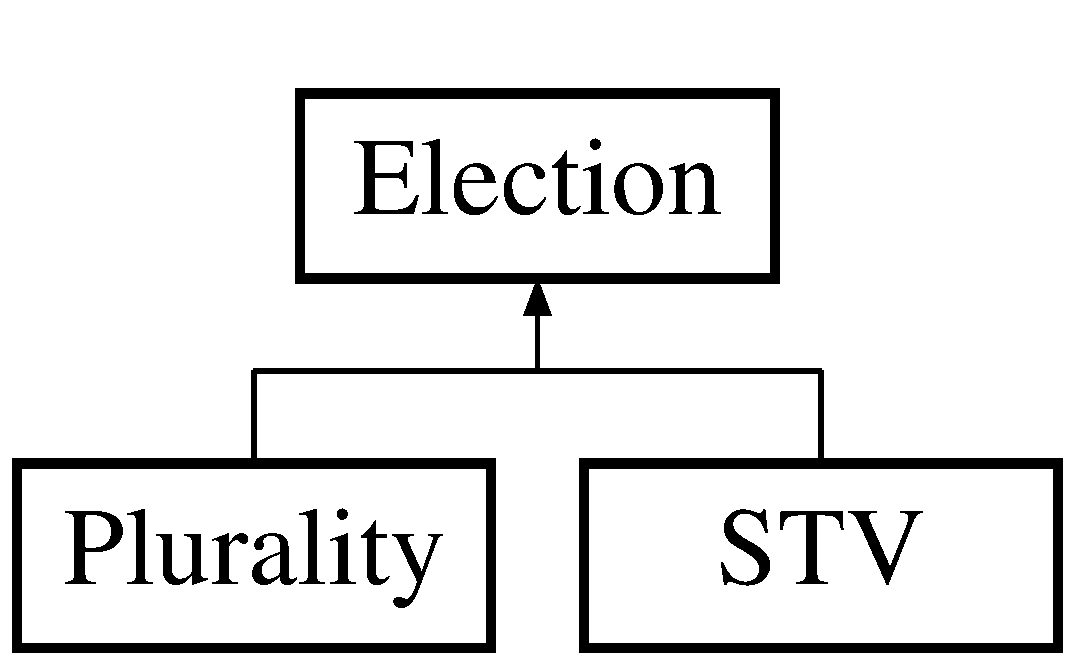
\includegraphics[height=2.000000cm]{class_election}
\end{center}
\end{figure}
\subsection*{Public Member Functions}
\begin{DoxyCompactItemize}
\item 
\hyperlink{class_election_af15999d79dbd51ad41380207a2fb0ba4}{Election} (int num\+\_\+seats, int num\+\_\+candidates, int num\+\_\+ballots)
\begin{DoxyCompactList}\small\item\em Creates an \hyperlink{class_election}{Election} instance that gets the number of seats available, number of cadidates running and number of ballots. \end{DoxyCompactList}\item 
int \hyperlink{class_election_a9582c81b6b89805f531197efb0e34db8}{get\+\_\+num\+\_\+seats} ()\hypertarget{class_election_a9582c81b6b89805f531197efb0e34db8}{}\label{class_election_a9582c81b6b89805f531197efb0e34db8}

\begin{DoxyCompactList}\small\item\em Gets the number of seats available. \end{DoxyCompactList}\item 
void \hyperlink{class_election_ad39320c11e6c6d5c95dc6128a2dd0a07}{set\+\_\+ballot\+\_\+no} (int s)
\begin{DoxyCompactList}\small\item\em Sets the number of seats available (s) to the local variable (num\+\_\+seats) to store the value of the number of seats available. \end{DoxyCompactList}\item 
int \hyperlink{class_election_aabeb70eb7aae4e60c6173b71e4218d96}{get\+\_\+num\+\_\+candidates} ()\hypertarget{class_election_aabeb70eb7aae4e60c6173b71e4218d96}{}\label{class_election_aabeb70eb7aae4e60c6173b71e4218d96}

\begin{DoxyCompactList}\small\item\em Gets the number of candidates running. \end{DoxyCompactList}\item 
void \hyperlink{class_election_ad73c41e88247a694c44370b4d28c04d0}{set\+\_\+num\+\_\+candidates} (int c)
\begin{DoxyCompactList}\small\item\em Sets the number of candidates (c) to the local variable (num\+\_\+candidates) to store the value of the number of candidates. \end{DoxyCompactList}\item 
int \hyperlink{class_election_a99f8cd6773f5c046b975eb39109cd123}{get\+\_\+num\+\_\+ballots} ()\hypertarget{class_election_a99f8cd6773f5c046b975eb39109cd123}{}\label{class_election_a99f8cd6773f5c046b975eb39109cd123}

\begin{DoxyCompactList}\small\item\em Gets the number of ballots. \end{DoxyCompactList}\item 
void \hyperlink{class_election_ae8f4cc654d20ae3677f01584a62d33d0}{set\+\_\+num\+\_\+ballots} (int b)
\begin{DoxyCompactList}\small\item\em Sets the number of ballots (b) to the local variable (num\+\_\+ballots) to store the value of the number of ballots for the election. \end{DoxyCompactList}\item 
string \hyperlink{class_election_ae8f6ee235effaf70966f2e603bbe90b3}{get\+\_\+election\+\_\+type} ()\hypertarget{class_election_ae8f6ee235effaf70966f2e603bbe90b3}{}\label{class_election_ae8f6ee235effaf70966f2e603bbe90b3}

\begin{DoxyCompactList}\small\item\em Gets the election type. \end{DoxyCompactList}\item 
void \hyperlink{class_election_a5d08c46134fa0e59988138258ab53eed}{set\+\_\+election\+\_\+type} (string s)
\begin{DoxyCompactList}\small\item\em Sets the election type (s) to the local variable (election\+\_\+type) to store the value of the election type for the election. \end{DoxyCompactList}\item 
\hyperlink{class_candidate_list}{Candidate\+List} \& \hyperlink{class_election_abb17fd9395b0931c5f635c2c0dd30427}{get\+\_\+candidates} ()\hypertarget{class_election_abb17fd9395b0931c5f635c2c0dd30427}{}\label{class_election_abb17fd9395b0931c5f635c2c0dd30427}

\begin{DoxyCompactList}\small\item\em Returns the list of candidates in election. \end{DoxyCompactList}\item 
void \hyperlink{class_election_a726cbdaaca392d54675954d6d86f10f0}{set\+\_\+votes} (\hyperlink{class_candidate_list}{Candidate\+List} cs)
\begin{DoxyCompactList}\small\item\em sets the candidatess to equal to the votes from the \hyperlink{class_candidate_list}{Candidate\+List} Class \end{DoxyCompactList}\item 
vector$<$ string $>$ {\bfseries get\+\_\+names} ()\hypertarget{class_election_a0100bf20e0c74b160867ac15d814a406}{}\label{class_election_a0100bf20e0c74b160867ac15d814a406}

\item 
\hyperlink{class_ballot_list}{Ballot\+List} \& \hyperlink{class_election_aff53e44590e75eabca7ca1f10f287c2a}{get\+\_\+ballots} ()\hypertarget{class_election_aff53e44590e75eabca7ca1f10f287c2a}{}\label{class_election_aff53e44590e75eabca7ca1f10f287c2a}

\begin{DoxyCompactList}\small\item\em Returns the list of ballots in the election. \end{DoxyCompactList}\item 
void \hyperlink{class_election_a4bf9c6eb717929f143ea89718cb09fe9}{set\+\_\+ballots} (\hyperlink{class_ballot_list}{Ballot\+List} bs)
\begin{DoxyCompactList}\small\item\em sets the ballots to equal to the ballots obtained from the \hyperlink{class_ballot_list}{Ballot\+List} (bs) \end{DoxyCompactList}\item 
void \hyperlink{class_election_a70752317f5b403a3e779b3bf2a8c91f6}{Log} ()\hypertarget{class_election_a70752317f5b403a3e779b3bf2a8c91f6}{}\label{class_election_a70752317f5b403a3e779b3bf2a8c91f6}

\begin{DoxyCompactList}\small\item\em Pushes a string to a log file. \end{DoxyCompactList}\item 
void \hyperlink{class_election_a769bc27e7ab0a091eee5d11f3b382032}{Display\+Results} ()\hypertarget{class_election_a769bc27e7ab0a091eee5d11f3b382032}{}\label{class_election_a769bc27e7ab0a091eee5d11f3b382032}

\begin{DoxyCompactList}\small\item\em Shows Result of \hyperlink{class_election}{Election}. \end{DoxyCompactList}\item 
void \hyperlink{class_election_ad9b7c2ce89047e79429c6ba00f428343}{Move\+Ballot} (int bal\+\_\+no, \hyperlink{class_ballot_list}{Ballot\+List} \&src, \hyperlink{class_ballot_list}{Ballot\+List} \&dst)
\begin{DoxyCompactList}\small\item\em Moves ballot from one place to another. \end{DoxyCompactList}\item 
void \hyperlink{class_election_ad8977ccd4118d7995bf286886759bbcf}{Read\+Names} (string filename)\hypertarget{class_election_ad8977ccd4118d7995bf286886759bbcf}{}\label{class_election_ad8977ccd4118d7995bf286886759bbcf}

\begin{DoxyCompactList}\small\item\em Reads the csv file to initialize the candidates. \end{DoxyCompactList}\item 
void \hyperlink{class_election_a7cdc9c089dfb557d8948f6af9fe650fd}{Read\+Parameters} (string filename)\hypertarget{class_election_a7cdc9c089dfb557d8948f6af9fe650fd}{}\label{class_election_a7cdc9c089dfb557d8948f6af9fe650fd}

\begin{DoxyCompactList}\small\item\em Reads the csv file to initialize the election parameters. \end{DoxyCompactList}\item 
\hyperlink{class_candidate_list}{Candidate\+List} \& {\bfseries get\+\_\+elected} ()\hypertarget{class_election_a4b5e266bd47407f7401825a00ddf9dfe}{}\label{class_election_a4b5e266bd47407f7401825a00ddf9dfe}

\item 
\hyperlink{class_candidate_list}{Candidate\+List} \& {\bfseries get\+\_\+non\+\_\+elected} ()\hypertarget{class_election_a30145af53c1a39812e9b4fc6e53ebeb0}{}\label{class_election_a30145af53c1a39812e9b4fc6e53ebeb0}

\end{DoxyCompactItemize}


\subsection{Detailed Description}
An object that receives information about the number of seats, candidates, and ballots. Likewise, the class will store objects of \hyperlink{class_candidate_list}{Candidate\+List} and \hyperlink{class_ballot_list}{Ballot\+List}. 

\subsection{Constructor \& Destructor Documentation}
\index{Election@{Election}!Election@{Election}}
\index{Election@{Election}!Election@{Election}}
\subsubsection[{\texorpdfstring{Election(int num\+\_\+seats, int num\+\_\+candidates, int num\+\_\+ballots)}{Election(int num_seats, int num_candidates, int num_ballots)}}]{\setlength{\rightskip}{0pt plus 5cm}Election\+::\+Election (
\begin{DoxyParamCaption}
\item[{int}]{num\+\_\+seats, }
\item[{int}]{num\+\_\+candidates, }
\item[{int}]{num\+\_\+ballots}
\end{DoxyParamCaption}
)}\hypertarget{class_election_af15999d79dbd51ad41380207a2fb0ba4}{}\label{class_election_af15999d79dbd51ad41380207a2fb0ba4}


Creates an \hyperlink{class_election}{Election} instance that gets the number of seats available, number of cadidates running and number of ballots. 


\begin{DoxyParams}{Parameters}
{\em num\+\_\+seats} & Gets the inputted value of number of seats available for the election.\\
\hline
{\em num\+\_\+cadidates} & Gets the value of number of candidates running.\\
\hline
{\em num\+\_\+ballots} & Gets the number of ballots there are in voting. \\
\hline
\end{DoxyParams}


\subsection{Member Function Documentation}
\index{Election@{Election}!Move\+Ballot@{Move\+Ballot}}
\index{Move\+Ballot@{Move\+Ballot}!Election@{Election}}
\subsubsection[{\texorpdfstring{Move\+Ballot(int bal\+\_\+no, Ballot\+List \&src, Ballot\+List \&dst)}{MoveBallot(int bal_no, BallotList &src, BallotList &dst)}}]{\setlength{\rightskip}{0pt plus 5cm}void Election\+::\+Move\+Ballot (
\begin{DoxyParamCaption}
\item[{int}]{bal\+\_\+no, }
\item[{{\bf Ballot\+List} \&}]{src, }
\item[{{\bf Ballot\+List} \&}]{dst}
\end{DoxyParamCaption}
)}\hypertarget{class_election_ad9b7c2ce89047e79429c6ba00f428343}{}\label{class_election_ad9b7c2ce89047e79429c6ba00f428343}


Moves ballot from one place to another. 


\begin{DoxyParams}{Parameters}
{\em bal\+\_\+no} & Variable to store the ballot number\\
\hline
{\em src} & The \hyperlink{class_ballot_list}{Ballot\+List} object passed in\\
\hline
{\em dst} & The \hyperlink{class_ballot_list}{Ballot\+List} object that the src will be stored in \\
\hline
\end{DoxyParams}
\index{Election@{Election}!set\+\_\+ballot\+\_\+no@{set\+\_\+ballot\+\_\+no}}
\index{set\+\_\+ballot\+\_\+no@{set\+\_\+ballot\+\_\+no}!Election@{Election}}
\subsubsection[{\texorpdfstring{set\+\_\+ballot\+\_\+no(int s)}{set_ballot_no(int s)}}]{\setlength{\rightskip}{0pt plus 5cm}void Election\+::set\+\_\+ballot\+\_\+no (
\begin{DoxyParamCaption}
\item[{int}]{s}
\end{DoxyParamCaption}
)\hspace{0.3cm}{\ttfamily [inline]}}\hypertarget{class_election_ad39320c11e6c6d5c95dc6128a2dd0a07}{}\label{class_election_ad39320c11e6c6d5c95dc6128a2dd0a07}


Sets the number of seats available (s) to the local variable (num\+\_\+seats) to store the value of the number of seats available. 


\begin{DoxyParams}{Parameters}
{\em s} & Store the number of seats available. \\
\hline
\end{DoxyParams}
\index{Election@{Election}!set\+\_\+ballots@{set\+\_\+ballots}}
\index{set\+\_\+ballots@{set\+\_\+ballots}!Election@{Election}}
\subsubsection[{\texorpdfstring{set\+\_\+ballots(\+Ballot\+List bs)}{set_ballots(BallotList bs)}}]{\setlength{\rightskip}{0pt plus 5cm}void Election\+::set\+\_\+ballots (
\begin{DoxyParamCaption}
\item[{{\bf Ballot\+List}}]{bs}
\end{DoxyParamCaption}
)\hspace{0.3cm}{\ttfamily [inline]}}\hypertarget{class_election_a4bf9c6eb717929f143ea89718cb09fe9}{}\label{class_election_a4bf9c6eb717929f143ea89718cb09fe9}


sets the ballots to equal to the ballots obtained from the \hyperlink{class_ballot_list}{Ballot\+List} (bs) 


\begin{DoxyParams}{Parameters}
{\em bs} & Variable to get the ballots fro m the \hyperlink{class_ballot_list}{Ballot\+List} \\
\hline
\end{DoxyParams}
\index{Election@{Election}!set\+\_\+election\+\_\+type@{set\+\_\+election\+\_\+type}}
\index{set\+\_\+election\+\_\+type@{set\+\_\+election\+\_\+type}!Election@{Election}}
\subsubsection[{\texorpdfstring{set\+\_\+election\+\_\+type(string s)}{set_election_type(string s)}}]{\setlength{\rightskip}{0pt plus 5cm}void Election\+::set\+\_\+election\+\_\+type (
\begin{DoxyParamCaption}
\item[{string}]{s}
\end{DoxyParamCaption}
)\hspace{0.3cm}{\ttfamily [inline]}}\hypertarget{class_election_a5d08c46134fa0e59988138258ab53eed}{}\label{class_election_a5d08c46134fa0e59988138258ab53eed}


Sets the election type (s) to the local variable (election\+\_\+type) to store the value of the election type for the election. 


\begin{DoxyParams}{Parameters}
{\em s} & Store the number of ballots \\
\hline
\end{DoxyParams}
\index{Election@{Election}!set\+\_\+num\+\_\+ballots@{set\+\_\+num\+\_\+ballots}}
\index{set\+\_\+num\+\_\+ballots@{set\+\_\+num\+\_\+ballots}!Election@{Election}}
\subsubsection[{\texorpdfstring{set\+\_\+num\+\_\+ballots(int b)}{set_num_ballots(int b)}}]{\setlength{\rightskip}{0pt plus 5cm}void Election\+::set\+\_\+num\+\_\+ballots (
\begin{DoxyParamCaption}
\item[{int}]{b}
\end{DoxyParamCaption}
)\hspace{0.3cm}{\ttfamily [inline]}}\hypertarget{class_election_ae8f4cc654d20ae3677f01584a62d33d0}{}\label{class_election_ae8f4cc654d20ae3677f01584a62d33d0}


Sets the number of ballots (b) to the local variable (num\+\_\+ballots) to store the value of the number of ballots for the election. 


\begin{DoxyParams}{Parameters}
{\em b} & Store the number of ballots \\
\hline
\end{DoxyParams}
\index{Election@{Election}!set\+\_\+num\+\_\+candidates@{set\+\_\+num\+\_\+candidates}}
\index{set\+\_\+num\+\_\+candidates@{set\+\_\+num\+\_\+candidates}!Election@{Election}}
\subsubsection[{\texorpdfstring{set\+\_\+num\+\_\+candidates(int c)}{set_num_candidates(int c)}}]{\setlength{\rightskip}{0pt plus 5cm}void Election\+::set\+\_\+num\+\_\+candidates (
\begin{DoxyParamCaption}
\item[{int}]{c}
\end{DoxyParamCaption}
)\hspace{0.3cm}{\ttfamily [inline]}}\hypertarget{class_election_ad73c41e88247a694c44370b4d28c04d0}{}\label{class_election_ad73c41e88247a694c44370b4d28c04d0}


Sets the number of candidates (c) to the local variable (num\+\_\+candidates) to store the value of the number of candidates. 


\begin{DoxyParams}{Parameters}
{\em c} & Store the number of canidates \\
\hline
\end{DoxyParams}
\index{Election@{Election}!set\+\_\+votes@{set\+\_\+votes}}
\index{set\+\_\+votes@{set\+\_\+votes}!Election@{Election}}
\subsubsection[{\texorpdfstring{set\+\_\+votes(\+Candidate\+List cs)}{set_votes(CandidateList cs)}}]{\setlength{\rightskip}{0pt plus 5cm}void Election\+::set\+\_\+votes (
\begin{DoxyParamCaption}
\item[{{\bf Candidate\+List}}]{cs}
\end{DoxyParamCaption}
)\hspace{0.3cm}{\ttfamily [inline]}}\hypertarget{class_election_a726cbdaaca392d54675954d6d86f10f0}{}\label{class_election_a726cbdaaca392d54675954d6d86f10f0}


sets the candidatess to equal to the votes from the \hyperlink{class_candidate_list}{Candidate\+List} Class 


\begin{DoxyParams}{Parameters}
{\em cs} & Variable to get the votes from the \hyperlink{class_candidate_list}{Candidate\+List} \\
\hline
\end{DoxyParams}


The documentation for this class was generated from the following files\+:\begin{DoxyCompactItemize}
\item 
include/Election.\+h\item 
src/Election.\+cc\end{DoxyCompactItemize}

\hypertarget{classmain}{}\section{main Class Reference}
\label{classmain}\index{main@{main}}


Main driver of the Voting System.  




{\ttfamily \#include $<$main.\+h$>$}



\subsection{Detailed Description}
Main driver of the Voting System. 

The documentation for this class was generated from the following file\+:\begin{DoxyCompactItemize}
\item 
include/main.\+h\end{DoxyCompactItemize}

\hypertarget{class_plurality}{}\section{Plurality Class Reference}
\label{class_plurality}\index{Plurality@{Plurality}}


The \hyperlink{class_plurality}{Plurality} class inherits from the \hyperlink{class_election}{Election} class. The class implements the \hyperlink{class_plurality}{Plurality} algorithm to identify the winning candidates.  




{\ttfamily \#include $<$Plurality.\+h$>$}

Inheritance diagram for Plurality\+:\begin{figure}[H]
\begin{center}
\leavevmode
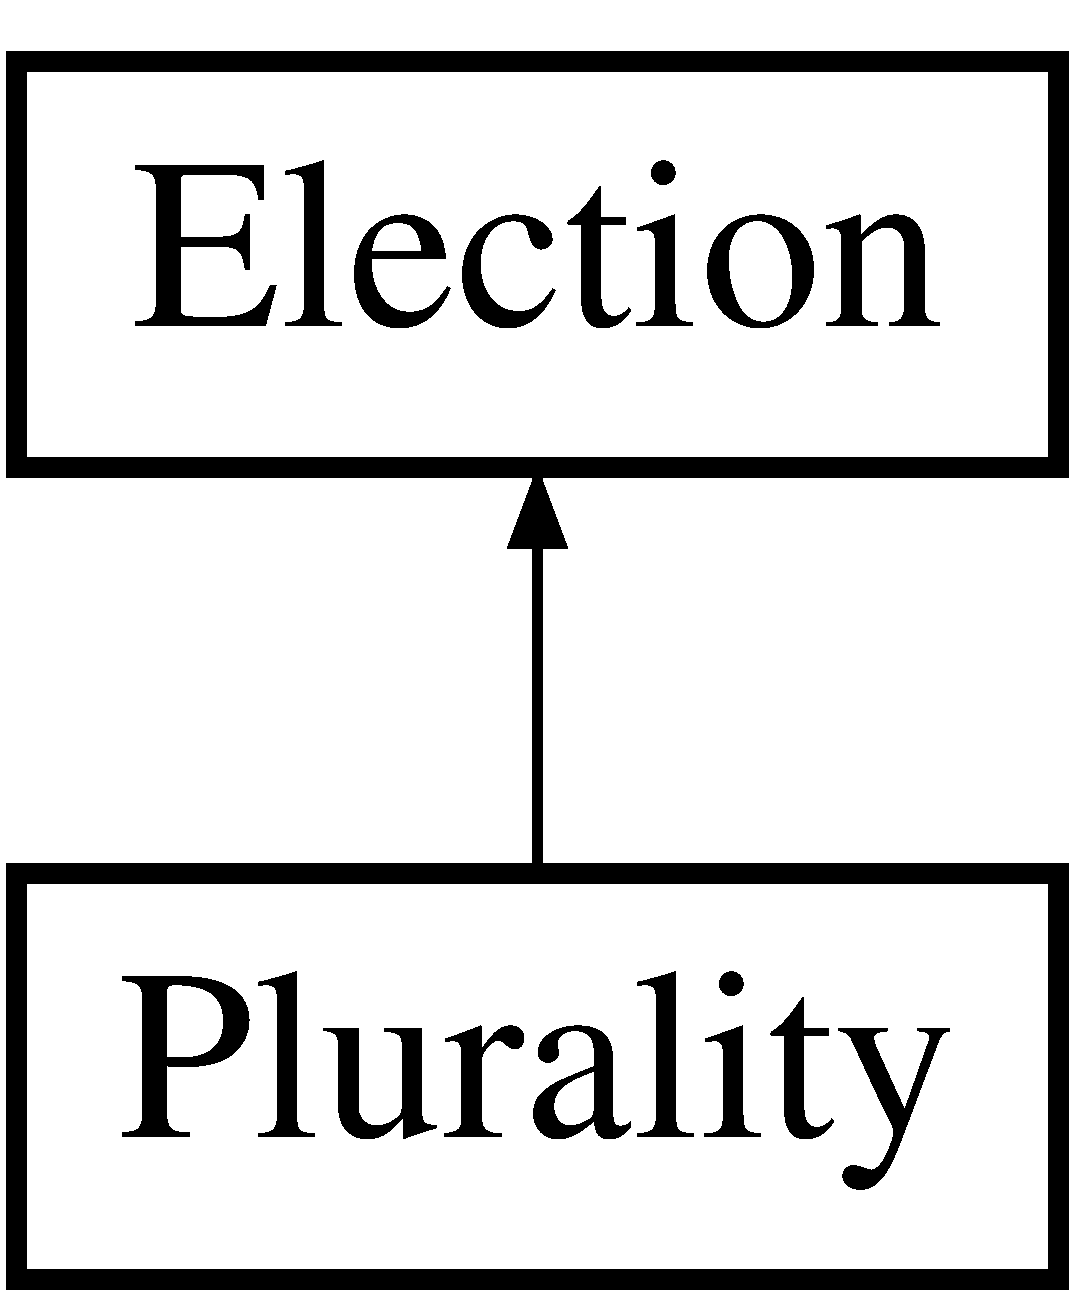
\includegraphics[height=2.000000cm]{class_plurality}
\end{center}
\end{figure}
\subsection*{Public Member Functions}
\begin{DoxyCompactItemize}
\item 
\hyperlink{class_plurality_a26d4ba756a5bfc0d5c8d40865e5ecbb8}{Plurality} ()\hypertarget{class_plurality_a26d4ba756a5bfc0d5c8d40865e5ecbb8}{}\label{class_plurality_a26d4ba756a5bfc0d5c8d40865e5ecbb8}

\begin{DoxyCompactList}\small\item\em Default constructor for \hyperlink{class_plurality}{Plurality}. \end{DoxyCompactList}\item 
\hyperlink{class_plurality_a4fc0116515730145cf4d4cfedbf34b1c}{Plurality} (int num\+\_\+seats, int num\+\_\+candidates, int num\+\_\+ballots)
\begin{DoxyCompactList}\small\item\em Constructor for \hyperlink{class_plurality}{Plurality}. \end{DoxyCompactList}\item 
void \hyperlink{class_plurality_a63b556aa77c6ea04f52a42fadc9474e8}{Algorithm} ()\hypertarget{class_plurality_a63b556aa77c6ea04f52a42fadc9474e8}{}\label{class_plurality_a63b556aa77c6ea04f52a42fadc9474e8}

\begin{DoxyCompactList}\small\item\em Main driver of the \hyperlink{class_plurality}{Plurality} voting. \end{DoxyCompactList}\item 
int \hyperlink{class_plurality_a9617e0aacc5e6fb714632f4657ee6576}{Return\+Highest\+Vote\+Index} (\hyperlink{class_ballot}{Ballot} b)
\begin{DoxyCompactList}\small\item\em Returns the index of the highest vote in a ballot. \end{DoxyCompactList}\end{DoxyCompactItemize}


\subsection{Detailed Description}
The \hyperlink{class_plurality}{Plurality} class inherits from the \hyperlink{class_election}{Election} class. The class implements the \hyperlink{class_plurality}{Plurality} algorithm to identify the winning candidates. 



 Name \+: \hyperlink{_plurality_8h_source}{Plurality.\+h} Project \+: Voting System Description \+: Header file for \hyperlink{class_plurality}{Plurality} Original Authors \+: Maxwell Dahl, Sanjana Jonnalagadda, Anthony Phan, Ronny Yogiswara



 Includes



 Class Definitions 

\subsection{Constructor \& Destructor Documentation}
\index{Plurality@{Plurality}!Plurality@{Plurality}}
\index{Plurality@{Plurality}!Plurality@{Plurality}}
\subsubsection[{\texorpdfstring{Plurality(int num\+\_\+seats, int num\+\_\+candidates, int num\+\_\+ballots)}{Plurality(int num_seats, int num_candidates, int num_ballots)}}]{\setlength{\rightskip}{0pt plus 5cm}Plurality\+::\+Plurality (
\begin{DoxyParamCaption}
\item[{int}]{num\+\_\+seats, }
\item[{int}]{num\+\_\+candidates, }
\item[{int}]{num\+\_\+ballots}
\end{DoxyParamCaption}
)}\hypertarget{class_plurality_a4fc0116515730145cf4d4cfedbf34b1c}{}\label{class_plurality_a4fc0116515730145cf4d4cfedbf34b1c}


Constructor for \hyperlink{class_plurality}{Plurality}. 


\begin{DoxyParams}{Parameters}
{\em num\+\_\+seats} & Number of available seats in election \\
\hline
{\em num\+\_\+candidates} & Number of total candidates in election \\
\hline
{\em num\+\_\+ballots} & Number of total ballots in election \\
\hline
\end{DoxyParams}


\subsection{Member Function Documentation}
\index{Plurality@{Plurality}!Return\+Highest\+Vote\+Index@{Return\+Highest\+Vote\+Index}}
\index{Return\+Highest\+Vote\+Index@{Return\+Highest\+Vote\+Index}!Plurality@{Plurality}}
\subsubsection[{\texorpdfstring{Return\+Highest\+Vote\+Index(\+Ballot b)}{ReturnHighestVoteIndex(Ballot b)}}]{\setlength{\rightskip}{0pt plus 5cm}int Plurality\+::\+Return\+Highest\+Vote\+Index (
\begin{DoxyParamCaption}
\item[{{\bf Ballot}}]{b}
\end{DoxyParamCaption}
)}\hypertarget{class_plurality_a9617e0aacc5e6fb714632f4657ee6576}{}\label{class_plurality_a9617e0aacc5e6fb714632f4657ee6576}


Returns the index of the highest vote in a ballot. 


\begin{DoxyParams}{Parameters}
{\em b} & \hyperlink{class_ballot}{Ballot} to read through. \\
\hline
\end{DoxyParams}


The documentation for this class was generated from the following files\+:\begin{DoxyCompactItemize}
\item 
include/Plurality.\+h\item 
src/Plurality.\+cc\end{DoxyCompactItemize}

\hypertarget{class_s_t_v}{}\section{S\+TV Class Reference}
\label{class_s_t_v}\index{S\+TV@{S\+TV}}


The \hyperlink{class_s_t_v}{S\+TV} class inherits from the \hyperlink{class_election}{Election} class. The class implements the \hyperlink{class_s_t_v}{S\+TV} algorithm to identify the winning candidates.  




{\ttfamily \#include $<$S\+T\+V.\+h$>$}

Inheritance diagram for S\+TV\+:\begin{figure}[H]
\begin{center}
\leavevmode
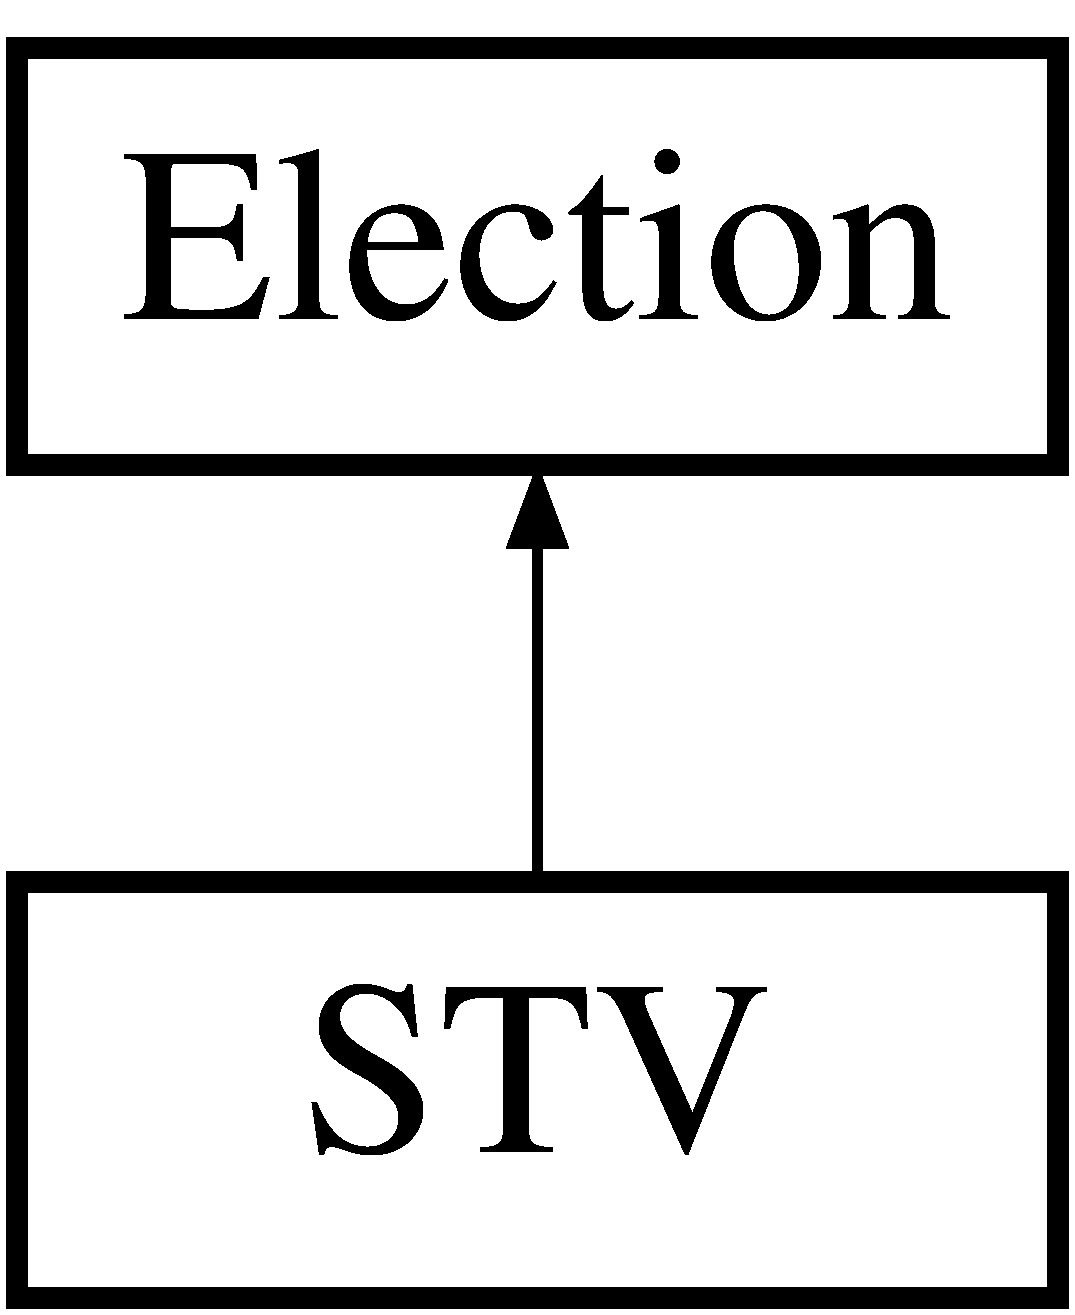
\includegraphics[height=2.000000cm]{class_s_t_v}
\end{center}
\end{figure}
\subsection*{Public Member Functions}
\begin{DoxyCompactItemize}
\item 
\hyperlink{class_s_t_v_a9ccdab1558b1936150844bbd506b4197}{S\+TV} ()
\begin{DoxyCompactList}\small\item\em Default constructor for \hyperlink{class_s_t_v}{S\+TV}./$\ast$$\ast$. \end{DoxyCompactList}\item 
\hyperlink{class_s_t_v_a07f1d636448505df93a855cf1c25c02a}{S\+TV} (int num\+\_\+seats, int num\+\_\+candidates, int num\+\_\+ballots)
\begin{DoxyCompactList}\small\item\em Constructor for \hyperlink{class_s_t_v}{S\+TV}. \end{DoxyCompactList}\item 
string \hyperlink{class_s_t_v_a05737f758ce07cce32067285d1b388b4}{Return\+Name\+Of\+Vote} (\hyperlink{class_ballot}{Ballot} b)
\begin{DoxyCompactList}\small\item\em Returns the name of candidate with the highest vote in a ballot. \end{DoxyCompactList}\item 
void \hyperlink{class_s_t_v_ac77d6adc39f384482f03ddd9b1977132}{Algorithm} ()\hypertarget{class_s_t_v_ac77d6adc39f384482f03ddd9b1977132}{}\label{class_s_t_v_ac77d6adc39f384482f03ddd9b1977132}

\begin{DoxyCompactList}\small\item\em Main driver of the \hyperlink{class_s_t_v}{S\+TV} voting. \end{DoxyCompactList}\item 
void \hyperlink{class_s_t_v_ac0253d507a1a4897385d0b1b1245beeb}{Calculate\+Droop} ()\hypertarget{class_s_t_v_ac0253d507a1a4897385d0b1b1245beeb}{}\label{class_s_t_v_ac0253d507a1a4897385d0b1b1245beeb}

\begin{DoxyCompactList}\small\item\em Calculates the Droop number for \hyperlink{class_s_t_v}{S\+TV}. \end{DoxyCompactList}\item 
void \hyperlink{class_s_t_v_ae905b9379a145c034f40428618668d57}{Move\+Candidate} (string can\+\_\+name, \hyperlink{class_candidate_list}{Candidate\+List} \&src, \hyperlink{class_candidate_list}{Candidate\+List} \&dst)
\begin{DoxyCompactList}\small\item\em Moves the candidate from one source location to the desitnation location. \end{DoxyCompactList}\item 
int \hyperlink{class_s_t_v_a63c8ba4b45b050ead77a884b1a21e534}{get\+\_\+droop} ()\hypertarget{class_s_t_v_a63c8ba4b45b050ead77a884b1a21e534}{}\label{class_s_t_v_a63c8ba4b45b050ead77a884b1a21e534}

\begin{DoxyCompactList}\small\item\em Retrieves the droop value. \end{DoxyCompactList}\item 
void \hyperlink{class_s_t_v_a3bb1ea48a3d11d9e02ee8d5892557bdd}{set\+\_\+droop} (int d)\hypertarget{class_s_t_v_a3bb1ea48a3d11d9e02ee8d5892557bdd}{}\label{class_s_t_v_a3bb1ea48a3d11d9e02ee8d5892557bdd}

\begin{DoxyCompactList}\small\item\em Returns the droop value. \end{DoxyCompactList}\item 
int \hyperlink{class_s_t_v_a28fcd1b404443f9fb1562a4343a44fb9}{get\+\_\+index} (vector$<$ int $>$ v, int n)
\begin{DoxyCompactList}\small\item\em Gets the index of the vector. \end{DoxyCompactList}\end{DoxyCompactItemize}


\subsection{Detailed Description}
The \hyperlink{class_s_t_v}{S\+TV} class inherits from the \hyperlink{class_election}{Election} class. The class implements the \hyperlink{class_s_t_v}{S\+TV} algorithm to identify the winning candidates. 



 Name \+: \hyperlink{_s_t_v_8h_source}{S\+T\+V.\+h} Project \+: Voting System Description \+: Header file for \hyperlink{class_s_t_v}{S\+TV} Original Authors \+: Maxwell Dahl, Sanjana Jonnalagadda, Anthony Phan, Ronny Yogiswara



 Includes



 Class Definitions 

\subsection{Constructor \& Destructor Documentation}
\index{S\+TV@{S\+TV}!S\+TV@{S\+TV}}
\index{S\+TV@{S\+TV}!S\+TV@{S\+TV}}
\subsubsection[{\texorpdfstring{S\+T\+V()}{STV()}}]{\setlength{\rightskip}{0pt plus 5cm}S\+T\+V\+::\+S\+TV (
\begin{DoxyParamCaption}
{}
\end{DoxyParamCaption}
)}\hypertarget{class_s_t_v_a9ccdab1558b1936150844bbd506b4197}{}\label{class_s_t_v_a9ccdab1558b1936150844bbd506b4197}


Default constructor for \hyperlink{class_s_t_v}{S\+TV}./$\ast$$\ast$. 

Calculates the Droop number for \hyperlink{class_s_t_v}{S\+TV}. \index{S\+TV@{S\+TV}!S\+TV@{S\+TV}}
\index{S\+TV@{S\+TV}!S\+TV@{S\+TV}}
\subsubsection[{\texorpdfstring{S\+T\+V(int num\+\_\+seats, int num\+\_\+candidates, int num\+\_\+ballots)}{STV(int num_seats, int num_candidates, int num_ballots)}}]{\setlength{\rightskip}{0pt plus 5cm}S\+T\+V\+::\+S\+TV (
\begin{DoxyParamCaption}
\item[{int}]{num\+\_\+seats, }
\item[{int}]{num\+\_\+candidates, }
\item[{int}]{num\+\_\+ballots}
\end{DoxyParamCaption}
)}\hypertarget{class_s_t_v_a07f1d636448505df93a855cf1c25c02a}{}\label{class_s_t_v_a07f1d636448505df93a855cf1c25c02a}


Constructor for \hyperlink{class_s_t_v}{S\+TV}. 


\begin{DoxyParams}{Parameters}
{\em num\+\_\+seats} & Number of available seats in election \\
\hline
{\em num\+\_\+candidates} & Number of total candidates in election \\
\hline
{\em num\+\_\+ballots} & Number of total ballots in election \\
\hline
\end{DoxyParams}


\subsection{Member Function Documentation}
\index{S\+TV@{S\+TV}!get\+\_\+index@{get\+\_\+index}}
\index{get\+\_\+index@{get\+\_\+index}!S\+TV@{S\+TV}}
\subsubsection[{\texorpdfstring{get\+\_\+index(vector$<$ int $>$ v, int n)}{get_index(vector< int > v, int n)}}]{\setlength{\rightskip}{0pt plus 5cm}int S\+T\+V\+::get\+\_\+index (
\begin{DoxyParamCaption}
\item[{vector$<$ int $>$}]{v, }
\item[{int}]{n}
\end{DoxyParamCaption}
)}\hypertarget{class_s_t_v_a28fcd1b404443f9fb1562a4343a44fb9}{}\label{class_s_t_v_a28fcd1b404443f9fb1562a4343a44fb9}


Gets the index of the vector. 


\begin{DoxyParams}{Parameters}
{\em v} & The vector list \\
\hline
{\em n} & The value of the index trying to look for \\
\hline
\end{DoxyParams}
\index{S\+TV@{S\+TV}!Move\+Candidate@{Move\+Candidate}}
\index{Move\+Candidate@{Move\+Candidate}!S\+TV@{S\+TV}}
\subsubsection[{\texorpdfstring{Move\+Candidate(string can\+\_\+name, Candidate\+List \&src, Candidate\+List \&dst)}{MoveCandidate(string can_name, CandidateList &src, CandidateList &dst)}}]{\setlength{\rightskip}{0pt plus 5cm}void S\+T\+V\+::\+Move\+Candidate (
\begin{DoxyParamCaption}
\item[{string}]{can\+\_\+name, }
\item[{{\bf Candidate\+List} \&}]{src, }
\item[{{\bf Candidate\+List} \&}]{dst}
\end{DoxyParamCaption}
)}\hypertarget{class_s_t_v_ae905b9379a145c034f40428618668d57}{}\label{class_s_t_v_ae905b9379a145c034f40428618668d57}


Moves the candidate from one source location to the desitnation location. 


\begin{DoxyParams}{Parameters}
{\em can\+\_\+name} & The \hyperlink{class_candidate}{Candidate} name \\
\hline
{\em src} & The source of the \hyperlink{class_candidate_list}{Candidate\+List} \\
\hline
{\em dst} & The destination of the \hyperlink{class_candidate_list}{Candidate\+List} when re-\/distributing votes \\
\hline
\end{DoxyParams}
\index{S\+TV@{S\+TV}!Return\+Name\+Of\+Vote@{Return\+Name\+Of\+Vote}}
\index{Return\+Name\+Of\+Vote@{Return\+Name\+Of\+Vote}!S\+TV@{S\+TV}}
\subsubsection[{\texorpdfstring{Return\+Name\+Of\+Vote(\+Ballot b)}{ReturnNameOfVote(Ballot b)}}]{\setlength{\rightskip}{0pt plus 5cm}string S\+T\+V\+::\+Return\+Name\+Of\+Vote (
\begin{DoxyParamCaption}
\item[{{\bf Ballot}}]{b}
\end{DoxyParamCaption}
)}\hypertarget{class_s_t_v_a05737f758ce07cce32067285d1b388b4}{}\label{class_s_t_v_a05737f758ce07cce32067285d1b388b4}


Returns the name of candidate with the highest vote in a ballot. 


\begin{DoxyParams}{Parameters}
{\em b} & \hyperlink{class_ballot}{Ballot} to read through. \\
\hline
\end{DoxyParams}


The documentation for this class was generated from the following files\+:\begin{DoxyCompactItemize}
\item 
include/S\+T\+V.\+h\item 
src/S\+T\+V.\+cc\end{DoxyCompactItemize}

%--- End generated contents ---

% Index
\backmatter
\newpage
\phantomsection
\clearemptydoublepage
\addcontentsline{toc}{chapter}{Index}
\printindex

\end{document}
